%*----------- SLIDE -------------------------------------------------------------
\begin{frame}[t]{Finalização}
    \begin{itemize}
        \item Cada líder deverá realizar a apresentação final do desafio no dia 25/maio/2020.
        \item No dia da apresentação, somente o líder poderá responder os questionamentos emitidos pelos facilitadores.
        \item A avaliação será da equipe, não havendo avaliação individual dos integrantes da equipe com exceção do líder de cada equipe.
        \item A apresentação deverá ser desenvolvida em latex.
        \item Os videos dos desafios deverão estar contidos na apresentação final.
        \item Os videos deverão ser completos, tendo começo, meio e fim da missão realizada.
    \end{itemize}
%*----------- notes
    \note[item]{Notes can help you to remember important information. Turn on the notes option.}
\end{frame}
%-
%*----------- SLIDE -------------------------------------------------------------
\begin{frame}[c]{A importância atual da robótica}
    \begin{center}
        % \movie[loop,width=0.6\linewidth,height=0.3375\linewidth,showcontrols=false,autostart]{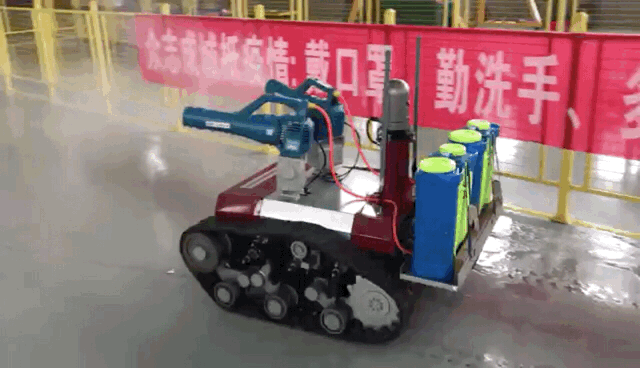
\includegraphics[width=0.6\textwidth]{Media/gifs/robotdesinfec0.png}}{Media/gifs/robotdesinfec.wmv}
    
        \includemedia[
            width=0.7\linewidth,
            totalheight=0.39375\linewidth,
            activate=pageopen,
            passcontext, 
            %transparent,
            addresource=./Media/gifs/robotdesinfec.wmv,
            flashvars={
            source=./Media/gifs/robotdesinfec.wmv
            &autoPlay=true
            &autoRewind=true
            &loop=true}
            ]{\fbox{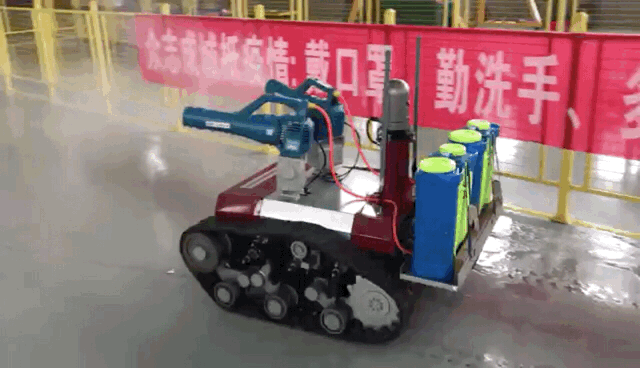
\includegraphics{Media/gifs/robotdesinfec0.png}}}{VPlayer.swf}
    \end{center}
%  %\movie[width=8cm,height=4.5cm]{test}{../Movies/Darwin-OP.mp4}

% % \includemedia[
% %     width=0.4\linewidth,
% %     totalheight=0.225\linewidth,
% %     activate=pageopen,
% %     passcontext,  %show VPlayer's right-click menu
% %     addresource=../Movies/Darwin-OP.mp4,
% %     flashvars={
% %       %important: same path as in `addresource'
% %       source=../Movies/Darwin-OP.mp4
% %     }
% %   ]{\fbox{Click!}}{VPlayer.swf}

%     \pdfpcmovie{\includegraphics[width=\textwidth]{Darwin-OP}}{Darwin-OP.mp4}

%*----------- notes
    \note[item]{Notes can help you to remember important information. Turn on the notes option.}
 \end{frame}
%-
%*----------- SLIDE -------------------------------------------------------------
\begin{frame}[fragile]{A importância atual da robótica}
    Para a implentação de R gráficos deve-se realizar os seguintes comando no ambiente R:
    \begin{lstlisting}[language=R]
        library(tikzDevice)
        beamer.parms = list(paperwidth   = 364.19536/72,
                    paperheight  = 273.14662/72,
                    textwidth    = 307.28987/72,
                    textheight   = 269.14662/72)
        tikz("./your_file.tex", 
            width = beamer.parms$textwidth, 
            height = beamer.parms$textheight)
        ggqqplot(na.omit(my_data$col2))
        dev.off()
    \end{lstlisting}

    \begin{columns}
        \column{.01\textwidth}
        \column{.59\textwidth}
            \textbf{A penúltima linha do texto acima é o códifo em R para a construção do gráfico.}
                
        \column{.4\textwidth}
            \centering
            \begin{tikzpicture}[thick, scale=0.4, every node/.style={scale=0.1}]
                \node[at=(current page.center)] {
               %% Created by tikzDevice version 0.12.3 on 2020-05-14 20:48:40
% !TEX encoding = UTF-8 Unicode
\begin{tikzpicture}[x=1pt,y=1pt]
\definecolor{fillColor}{RGB}{255,255,255}
\path[use as bounding box,fill=fillColor,fill opacity=0.00] (0,0) rectangle (308.44,270.16);
\begin{scope}
\path[clip] (  0.00,  0.00) rectangle (308.44,270.16);
\definecolor{drawColor}{RGB}{255,255,255}
\definecolor{fillColor}{RGB}{255,255,255}

\path[draw=drawColor,line width= 0.6pt,line join=round,line cap=round,fill=fillColor] (  0.00,  0.00) rectangle (308.44,270.16);
\end{scope}
\begin{scope}
\path[clip] ( 36.99, 35.59) rectangle (302.44,264.16);
\definecolor{fillColor}{RGB}{255,255,255}

\path[fill=fillColor] ( 36.99, 35.59) rectangle (302.44,264.16);
\definecolor{drawColor}{RGB}{0,0,0}
\definecolor{fillColor}{RGB}{0,0,0}

\path[draw=drawColor,line width= 0.4pt,line join=round,line cap=round,fill=fillColor] ( 49.06, 83.70) circle (  1.96);

\path[draw=drawColor,line width= 0.4pt,line join=round,line cap=round,fill=fillColor] ( 78.84, 92.35) circle (  1.96);

\path[draw=drawColor,line width= 0.4pt,line join=round,line cap=round,fill=fillColor] ( 95.19,107.92) circle (  1.96);

\path[draw=drawColor,line width= 0.4pt,line join=round,line cap=round,fill=fillColor] (107.25,111.38) circle (  1.96);

\path[draw=drawColor,line width= 0.4pt,line join=round,line cap=round,fill=fillColor] (117.17,121.76) circle (  1.96);

\path[draw=drawColor,line width= 0.4pt,line join=round,line cap=round,fill=fillColor] (125.79,125.22) circle (  1.96);

\path[draw=drawColor,line width= 0.4pt,line join=round,line cap=round,fill=fillColor] (133.57,128.68) circle (  1.96);

\path[draw=drawColor,line width= 0.4pt,line join=round,line cap=round,fill=fillColor] (140.76,132.14) circle (  1.96);

\path[draw=drawColor,line width= 0.4pt,line join=round,line cap=round,fill=fillColor] (147.56,133.87) circle (  1.96);

\path[draw=drawColor,line width= 0.4pt,line join=round,line cap=round,fill=fillColor] (154.07,137.33) circle (  1.96);

\path[draw=drawColor,line width= 0.4pt,line join=round,line cap=round,fill=fillColor] (160.40,142.52) circle (  1.96);

\path[draw=drawColor,line width= 0.4pt,line join=round,line cap=round,fill=fillColor] (166.62,142.52) circle (  1.96);

\path[draw=drawColor,line width= 0.4pt,line join=round,line cap=round,fill=fillColor] (172.81,145.98) circle (  1.96);

\path[draw=drawColor,line width= 0.4pt,line join=round,line cap=round,fill=fillColor] (179.04,149.44) circle (  1.96);

\path[draw=drawColor,line width= 0.4pt,line join=round,line cap=round,fill=fillColor] (185.37,159.82) circle (  1.96);

\path[draw=drawColor,line width= 0.4pt,line join=round,line cap=round,fill=fillColor] (191.88,161.55) circle (  1.96);

\path[draw=drawColor,line width= 0.4pt,line join=round,line cap=round,fill=fillColor] (198.67,165.01) circle (  1.96);

\path[draw=drawColor,line width= 0.4pt,line join=round,line cap=round,fill=fillColor] (205.87,170.20) circle (  1.96);

\path[draw=drawColor,line width= 0.4pt,line join=round,line cap=round,fill=fillColor] (213.65,177.12) circle (  1.96);

\path[draw=drawColor,line width= 0.4pt,line join=round,line cap=round,fill=fillColor] (222.27,177.12) circle (  1.96);

\path[draw=drawColor,line width= 0.4pt,line join=round,line cap=round,fill=fillColor] (232.18,180.58) circle (  1.96);

\path[draw=drawColor,line width= 0.4pt,line join=round,line cap=round,fill=fillColor] (244.25,182.31) circle (  1.96);

\path[draw=drawColor,line width= 0.4pt,line join=round,line cap=round,fill=fillColor] (260.60,187.50) circle (  1.96);

\path[draw=drawColor,line width= 0.4pt,line join=round,line cap=round,fill=fillColor] (290.38,190.96) circle (  1.96);

\path[draw=drawColor,line width= 0.6pt,line join=round] ( 49.06, 83.27) --
	( 78.84, 99.71) --
	( 95.19,108.73) --
	(107.25,115.39) --
	(117.17,120.86) --
	(125.79,125.62) --
	(133.57,129.92) --
	(140.76,133.89) --
	(147.56,137.64) --
	(154.07,141.24) --
	(160.40,144.73) --
	(166.62,148.17) --
	(172.81,151.58) --
	(179.04,155.02) --
	(185.37,158.51) --
	(191.88,162.11) --
	(198.67,165.86) --
	(205.87,169.83) --
	(213.65,174.13) --
	(222.27,178.89) --
	(232.18,184.36) --
	(244.25,191.02) --
	(260.60,200.04) --
	(290.38,216.48);
\definecolor{fillColor}{RGB}{0,0,0}

\path[fill=fillColor,fill opacity=0.20] ( 49.06,120.55) --
	( 78.84,125.46) --
	( 95.19,130.84) --
	(107.25,135.57) --
	(117.17,139.84) --
	(125.79,143.77) --
	(133.57,147.47) --
	(140.76,151.02) --
	(147.56,154.46) --
	(154.07,157.84) --
	(160.40,161.20) --
	(166.62,164.57) --
	(172.81,167.99) --
	(179.04,171.49) --
	(185.37,175.12) --
	(191.88,178.93) --
	(198.67,182.99) --
	(205.87,187.39) --
	(213.65,192.27) --
	(222.27,197.86) --
	(232.18,204.54) --
	(244.25,213.13) --
	(260.60,225.80) --
	(290.38,253.77) --
	(290.38,179.20) --
	(260.60,174.29) --
	(244.25,168.91) --
	(232.18,164.18) --
	(222.27,159.91) --
	(213.65,155.98) --
	(205.87,152.28) --
	(198.67,148.73) --
	(191.88,145.29) --
	(185.37,141.91) --
	(179.04,138.55) --
	(172.81,135.18) --
	(166.62,131.76) --
	(160.40,128.26) --
	(154.07,124.63) --
	(147.56,120.82) --
	(140.76,116.76) --
	(133.57,112.36) --
	(125.79,107.48) --
	(117.17,101.89) --
	(107.25, 95.21) --
	( 95.19, 86.62) --
	( 78.84, 73.95) --
	( 49.06, 45.98) --
	cycle;

\path[] ( 49.06,120.55) --
	( 78.84,125.46) --
	( 95.19,130.84) --
	(107.25,135.57) --
	(117.17,139.84) --
	(125.79,143.77) --
	(133.57,147.47) --
	(140.76,151.02) --
	(147.56,154.46) --
	(154.07,157.84) --
	(160.40,161.20) --
	(166.62,164.57) --
	(172.81,167.99) --
	(179.04,171.49) --
	(185.37,175.12) --
	(191.88,178.93) --
	(198.67,182.99) --
	(205.87,187.39) --
	(213.65,192.27) --
	(222.27,197.86) --
	(232.18,204.54) --
	(244.25,213.13) --
	(260.60,225.80) --
	(290.38,253.77);

\path[] (290.38,179.20) --
	(260.60,174.29) --
	(244.25,168.91) --
	(232.18,164.18) --
	(222.27,159.91) --
	(213.65,155.98) --
	(205.87,152.28) --
	(198.67,148.73) --
	(191.88,145.29) --
	(185.37,141.91) --
	(179.04,138.55) --
	(172.81,135.18) --
	(166.62,131.76) --
	(160.40,128.26) --
	(154.07,124.63) --
	(147.56,120.82) --
	(140.76,116.76) --
	(133.57,112.36) --
	(125.79,107.48) --
	(117.17,101.89) --
	(107.25, 95.21) --
	( 95.19, 86.62) --
	( 78.84, 73.95) --
	( 49.06, 45.98);
\end{scope}
\begin{scope}
\path[clip] (  0.00,  0.00) rectangle (308.44,270.16);
\definecolor{drawColor}{RGB}{0,0,0}

\path[draw=drawColor,line width= 0.6pt,line join=round] ( 36.99, 35.59) --
	( 36.99,264.16);
\end{scope}
\begin{scope}
\path[clip] (  0.00,  0.00) rectangle (308.44,270.16);
\definecolor{drawColor}{RGB}{0,0,0}

\node[text=drawColor,anchor=base east,inner sep=0pt, outer sep=0pt, scale=  1.20] at ( 31.59, 62.27) {40};

\node[text=drawColor,anchor=base east,inner sep=0pt, outer sep=0pt, scale=  1.20] at ( 31.59,131.47) {60};

\node[text=drawColor,anchor=base east,inner sep=0pt, outer sep=0pt, scale=  1.20] at ( 31.59,200.67) {80};
\end{scope}
\begin{scope}
\path[clip] (  0.00,  0.00) rectangle (308.44,270.16);
\definecolor{drawColor}{RGB}{0,0,0}

\path[draw=drawColor,line width= 0.6pt,line join=round] ( 33.99, 66.40) --
	( 36.99, 66.40);

\path[draw=drawColor,line width= 0.6pt,line join=round] ( 33.99,135.60) --
	( 36.99,135.60);

\path[draw=drawColor,line width= 0.6pt,line join=round] ( 33.99,204.80) --
	( 36.99,204.80);
\end{scope}
\begin{scope}
\path[clip] (  0.00,  0.00) rectangle (308.44,270.16);
\definecolor{drawColor}{RGB}{0,0,0}

\path[draw=drawColor,line width= 0.6pt,line join=round] ( 36.99, 35.59) --
	(302.44, 35.59);
\end{scope}
\begin{scope}
\path[clip] (  0.00,  0.00) rectangle (308.44,270.16);
\definecolor{drawColor}{RGB}{0,0,0}

\path[draw=drawColor,line width= 0.6pt,line join=round] ( 51.24, 32.59) --
	( 51.24, 35.59);

\path[draw=drawColor,line width= 0.6pt,line join=round] (110.48, 32.59) --
	(110.48, 35.59);

\path[draw=drawColor,line width= 0.6pt,line join=round] (169.72, 32.59) --
	(169.72, 35.59);

\path[draw=drawColor,line width= 0.6pt,line join=round] (228.96, 32.59) --
	(228.96, 35.59);

\path[draw=drawColor,line width= 0.6pt,line join=round] (288.19, 32.59) --
	(288.19, 35.59);
\end{scope}
\begin{scope}
\path[clip] (  0.00,  0.00) rectangle (308.44,270.16);
\definecolor{drawColor}{RGB}{0,0,0}

\node[text=drawColor,anchor=base,inner sep=0pt, outer sep=0pt, scale=  1.20] at ( 51.24, 21.93) {-2};

\node[text=drawColor,anchor=base,inner sep=0pt, outer sep=0pt, scale=  1.20] at (110.48, 21.93) {-1};

\node[text=drawColor,anchor=base,inner sep=0pt, outer sep=0pt, scale=  1.20] at (169.72, 21.93) {0};

\node[text=drawColor,anchor=base,inner sep=0pt, outer sep=0pt, scale=  1.20] at (228.96, 21.93) {1};

\node[text=drawColor,anchor=base,inner sep=0pt, outer sep=0pt, scale=  1.20] at (288.19, 21.93) {2};
\end{scope}
\begin{scope}
\path[clip] (  0.00,  0.00) rectangle (308.44,270.16);
\definecolor{drawColor}{RGB}{0,0,0}

\node[text=drawColor,anchor=base,inner sep=0pt, outer sep=0pt, scale=  1.20] at (169.72,  8.33) {Theoretical};
\end{scope}
\begin{scope}
\path[clip] (  0.00,  0.00) rectangle (308.44,270.16);
\definecolor{drawColor}{RGB}{0,0,0}

\node[text=drawColor,rotate= 90.00,anchor=base,inner sep=0pt, outer sep=0pt, scale=  1.20] at ( 14.26,149.88) {Sample};
\end{scope}
\end{tikzpicture}

                % Created by tikzDevice version 0.12.3 on 2020-05-19 09:32:09
% !TEX encoding = UTF-8 Unicode
\begin{tikzpicture}[x=1pt,y=1pt]
\definecolor{fillColor}{RGB}{255,255,255}
\path[use as bounding box,fill=fillColor,fill opacity=0.00] (0,0) rectangle (308.44,270.16);
\begin{scope}
\path[clip] ( 49.20, 61.20) rectangle (283.24,220.96);
\definecolor{drawColor}{RGB}{0,0,0}

\path[draw=drawColor,line width= 0.4pt,dash pattern=on 4pt off 4pt ,line join=round,line cap=round] ( 57.87, 67.12) --
	( 60.04, 67.14) --
	( 62.20, 67.16) --
	( 64.37, 67.19) --
	( 66.54, 67.24) --
	( 68.70, 67.29) --
	( 70.87, 67.37) --
	( 73.04, 67.47) --
	( 75.20, 67.59) --
	( 77.37, 67.75) --
	( 79.54, 67.95) --
	( 81.71, 68.21) --
	( 83.87, 68.52) --
	( 86.04, 68.92) --
	( 88.21, 69.41) --
	( 90.37, 70.00) --
	( 92.54, 70.73) --
	( 94.71, 71.60) --
	( 96.88, 72.65) --
	( 99.04, 73.90) --
	(101.21, 75.37) --
	(103.38, 77.10) --
	(105.54, 79.11) --
	(107.71, 81.42) --
	(109.88, 84.08) --
	(112.04, 87.09) --
	(114.21, 90.49) --
	(116.38, 94.29) --
	(118.55, 98.51) --
	(120.71,103.15) --
	(122.88,108.21) --
	(125.05,113.68) --
	(127.21,119.54) --
	(129.38,125.75) --
	(131.55,132.29) --
	(133.72,139.09) --
	(135.88,146.10) --
	(138.05,153.23) --
	(140.22,160.40) --
	(142.38,167.53) --
	(144.55,174.52) --
	(146.72,181.25) --
	(148.88,187.64) --
	(151.05,193.56) --
	(153.22,198.94) --
	(155.39,203.66) --
	(157.55,207.65) --
	(159.72,210.84) --
	(161.89,213.16) --
	(164.05,214.57) --
	(166.22,215.04) --
	(168.39,214.57) --
	(170.56,213.16) --
	(172.72,210.84) --
	(174.89,207.65) --
	(177.06,203.66) --
	(179.22,198.94) --
	(181.39,193.56) --
	(183.56,187.64) --
	(185.72,181.25) --
	(187.89,174.52) --
	(190.06,167.53) --
	(192.23,160.40) --
	(194.39,153.23) --
	(196.56,146.10) --
	(198.73,139.09) --
	(200.89,132.29) --
	(203.06,125.75) --
	(205.23,119.54) --
	(207.40,113.68) --
	(209.56,108.21) --
	(211.73,103.15) --
	(213.90, 98.51) --
	(216.06, 94.29) --
	(218.23, 90.49) --
	(220.40, 87.09) --
	(222.56, 84.08) --
	(224.73, 81.42) --
	(226.90, 79.11) --
	(229.07, 77.10) --
	(231.23, 75.37) --
	(233.40, 73.90) --
	(235.57, 72.65) --
	(237.73, 71.60) --
	(239.90, 70.73) --
	(242.07, 70.00) --
	(244.24, 69.41) --
	(246.40, 68.92) --
	(248.57, 68.52) --
	(250.74, 68.21) --
	(252.90, 67.95) --
	(255.07, 67.75) --
	(257.24, 67.59) --
	(259.40, 67.47) --
	(261.57, 67.37) --
	(263.74, 67.29) --
	(265.91, 67.24) --
	(268.07, 67.19) --
	(270.24, 67.16) --
	(272.41, 67.14) --
	(274.57, 67.12);
\end{scope}
\begin{scope}
\path[clip] (  0.00,  0.00) rectangle (308.44,270.16);
\definecolor{drawColor}{RGB}{0,0,0}

\node[text=drawColor,anchor=base,inner sep=0pt, outer sep=0pt, scale=  1.00] at (166.22, 15.60) {Observed value of the characteristic};

\node[text=drawColor,rotate= 90.00,anchor=base,inner sep=0pt, outer sep=0pt, scale=  1.00] at ( 10.80,141.08) {frequency};
\end{scope}
\begin{scope}
\path[clip] (  0.00,  0.00) rectangle (308.44,270.16);
\definecolor{drawColor}{RGB}{0,0,0}

\path[draw=drawColor,line width= 0.4pt,line join=round,line cap=round] ( 57.87, 61.20) -- (274.57, 61.20);

\path[draw=drawColor,line width= 0.4pt,line join=round,line cap=round] ( 57.87, 61.20) -- ( 57.87, 55.20);

\path[draw=drawColor,line width= 0.4pt,line join=round,line cap=round] (112.04, 61.20) -- (112.04, 55.20);

\path[draw=drawColor,line width= 0.4pt,line join=round,line cap=round] (166.22, 61.20) -- (166.22, 55.20);

\path[draw=drawColor,line width= 0.4pt,line join=round,line cap=round] (220.40, 61.20) -- (220.40, 55.20);

\path[draw=drawColor,line width= 0.4pt,line join=round,line cap=round] (274.57, 61.20) -- (274.57, 55.20);

\path[draw=drawColor,line width= 0.4pt,line join=round,line cap=round] ( 49.20, 67.07) -- ( 49.20,215.43);

\path[draw=drawColor,line width= 0.4pt,line join=round,line cap=round] ( 49.20, 67.07) -- ( 43.20, 67.07);

\path[draw=drawColor,line width= 0.4pt,line join=round,line cap=round] ( 49.20,104.16) -- ( 43.20,104.16);

\path[draw=drawColor,line width= 0.4pt,line join=round,line cap=round] ( 49.20,141.25) -- ( 43.20,141.25);

\path[draw=drawColor,line width= 0.4pt,line join=round,line cap=round] ( 49.20,178.34) -- ( 43.20,178.34);

\path[draw=drawColor,line width= 0.4pt,line join=round,line cap=round] ( 49.20,215.43) -- ( 43.20,215.43);
\end{scope}
\begin{scope}
\path[clip] ( 49.20, 61.20) rectangle (283.24,220.96);
\definecolor{drawColor}{RGB}{0,0,0}

\path[draw=drawColor,line width= 0.4pt,line join=round,line cap=round] (247.49, 61.20) -- (247.49,220.96);

\path[draw=drawColor,line width= 0.4pt,line join=round,line cap=round] ( 84.96, 61.20) -- ( 84.96,220.96);

\path[draw=drawColor,line width= 0.4pt,line join=round,line cap=round] (166.22, 61.20) -- (166.22,220.96);

\path[draw=drawColor,line width= 0.4pt,line join=round,line cap=round] ( 49.20, 67.07) -- (283.24, 67.07);

\node[text=drawColor,anchor=base,inner sep=0pt, outer sep=0pt, scale=  1.00] at (171.64,174.90) {T};

\node[text=drawColor,anchor=base,inner sep=0pt, outer sep=0pt, scale=  1.00] at (101.21,174.90) {LSL};

\node[text=drawColor,anchor=base,inner sep=0pt, outer sep=0pt, scale=  1.00] at (263.74,174.90) {USL};

\node[text=drawColor,anchor=base,inner sep=0pt, outer sep=0pt, scale=  1.00] at (220.40,100.71) {Variation};
\end{scope}
\begin{scope}
\path[clip] (  0.00,  0.00) rectangle (308.44,270.16);
\definecolor{drawColor}{RGB}{0,0,0}

\path[draw=drawColor,line width= 0.4pt,line join=round,line cap=round] (  0.00,  0.00) --
	(308.44,  0.00) --
	(308.44,270.16) --
	(  0.00,270.16) --
	(  0.00,  0.00);
\end{scope}
\end{tikzpicture}

                };
            \end{tikzpicture}
    \end{columns}
%*----------- notes
    \note[item]{Notes can help you to remember important information. Turn on the notes option.}
 \end{frame}
%-
%*----------- SLIDE -------------------------------------------------------------
\begin{frame}[c]{A importância atual da robótica}
    \centering
    \begin{tikzpicture}[thick, scale=0.4, every node/.style={scale=0.7}]
        \node[at=(current page.center)] {
        % Created by tikzDevice version 0.12.3 on 2020-05-19 09:32:09
% !TEX encoding = UTF-8 Unicode
\begin{tikzpicture}[x=1pt,y=1pt]
\definecolor{fillColor}{RGB}{255,255,255}
\path[use as bounding box,fill=fillColor,fill opacity=0.00] (0,0) rectangle (308.44,270.16);
\begin{scope}
\path[clip] ( 49.20, 61.20) rectangle (283.24,220.96);
\definecolor{drawColor}{RGB}{0,0,0}

\path[draw=drawColor,line width= 0.4pt,dash pattern=on 4pt off 4pt ,line join=round,line cap=round] ( 57.87, 67.12) --
	( 60.04, 67.14) --
	( 62.20, 67.16) --
	( 64.37, 67.19) --
	( 66.54, 67.24) --
	( 68.70, 67.29) --
	( 70.87, 67.37) --
	( 73.04, 67.47) --
	( 75.20, 67.59) --
	( 77.37, 67.75) --
	( 79.54, 67.95) --
	( 81.71, 68.21) --
	( 83.87, 68.52) --
	( 86.04, 68.92) --
	( 88.21, 69.41) --
	( 90.37, 70.00) --
	( 92.54, 70.73) --
	( 94.71, 71.60) --
	( 96.88, 72.65) --
	( 99.04, 73.90) --
	(101.21, 75.37) --
	(103.38, 77.10) --
	(105.54, 79.11) --
	(107.71, 81.42) --
	(109.88, 84.08) --
	(112.04, 87.09) --
	(114.21, 90.49) --
	(116.38, 94.29) --
	(118.55, 98.51) --
	(120.71,103.15) --
	(122.88,108.21) --
	(125.05,113.68) --
	(127.21,119.54) --
	(129.38,125.75) --
	(131.55,132.29) --
	(133.72,139.09) --
	(135.88,146.10) --
	(138.05,153.23) --
	(140.22,160.40) --
	(142.38,167.53) --
	(144.55,174.52) --
	(146.72,181.25) --
	(148.88,187.64) --
	(151.05,193.56) --
	(153.22,198.94) --
	(155.39,203.66) --
	(157.55,207.65) --
	(159.72,210.84) --
	(161.89,213.16) --
	(164.05,214.57) --
	(166.22,215.04) --
	(168.39,214.57) --
	(170.56,213.16) --
	(172.72,210.84) --
	(174.89,207.65) --
	(177.06,203.66) --
	(179.22,198.94) --
	(181.39,193.56) --
	(183.56,187.64) --
	(185.72,181.25) --
	(187.89,174.52) --
	(190.06,167.53) --
	(192.23,160.40) --
	(194.39,153.23) --
	(196.56,146.10) --
	(198.73,139.09) --
	(200.89,132.29) --
	(203.06,125.75) --
	(205.23,119.54) --
	(207.40,113.68) --
	(209.56,108.21) --
	(211.73,103.15) --
	(213.90, 98.51) --
	(216.06, 94.29) --
	(218.23, 90.49) --
	(220.40, 87.09) --
	(222.56, 84.08) --
	(224.73, 81.42) --
	(226.90, 79.11) --
	(229.07, 77.10) --
	(231.23, 75.37) --
	(233.40, 73.90) --
	(235.57, 72.65) --
	(237.73, 71.60) --
	(239.90, 70.73) --
	(242.07, 70.00) --
	(244.24, 69.41) --
	(246.40, 68.92) --
	(248.57, 68.52) --
	(250.74, 68.21) --
	(252.90, 67.95) --
	(255.07, 67.75) --
	(257.24, 67.59) --
	(259.40, 67.47) --
	(261.57, 67.37) --
	(263.74, 67.29) --
	(265.91, 67.24) --
	(268.07, 67.19) --
	(270.24, 67.16) --
	(272.41, 67.14) --
	(274.57, 67.12);
\end{scope}
\begin{scope}
\path[clip] (  0.00,  0.00) rectangle (308.44,270.16);
\definecolor{drawColor}{RGB}{0,0,0}

\node[text=drawColor,anchor=base,inner sep=0pt, outer sep=0pt, scale=  1.00] at (166.22, 15.60) {Observed value of the characteristic};

\node[text=drawColor,rotate= 90.00,anchor=base,inner sep=0pt, outer sep=0pt, scale=  1.00] at ( 10.80,141.08) {frequency};
\end{scope}
\begin{scope}
\path[clip] (  0.00,  0.00) rectangle (308.44,270.16);
\definecolor{drawColor}{RGB}{0,0,0}

\path[draw=drawColor,line width= 0.4pt,line join=round,line cap=round] ( 57.87, 61.20) -- (274.57, 61.20);

\path[draw=drawColor,line width= 0.4pt,line join=round,line cap=round] ( 57.87, 61.20) -- ( 57.87, 55.20);

\path[draw=drawColor,line width= 0.4pt,line join=round,line cap=round] (112.04, 61.20) -- (112.04, 55.20);

\path[draw=drawColor,line width= 0.4pt,line join=round,line cap=round] (166.22, 61.20) -- (166.22, 55.20);

\path[draw=drawColor,line width= 0.4pt,line join=round,line cap=round] (220.40, 61.20) -- (220.40, 55.20);

\path[draw=drawColor,line width= 0.4pt,line join=round,line cap=round] (274.57, 61.20) -- (274.57, 55.20);

\path[draw=drawColor,line width= 0.4pt,line join=round,line cap=round] ( 49.20, 67.07) -- ( 49.20,215.43);

\path[draw=drawColor,line width= 0.4pt,line join=round,line cap=round] ( 49.20, 67.07) -- ( 43.20, 67.07);

\path[draw=drawColor,line width= 0.4pt,line join=round,line cap=round] ( 49.20,104.16) -- ( 43.20,104.16);

\path[draw=drawColor,line width= 0.4pt,line join=round,line cap=round] ( 49.20,141.25) -- ( 43.20,141.25);

\path[draw=drawColor,line width= 0.4pt,line join=round,line cap=round] ( 49.20,178.34) -- ( 43.20,178.34);

\path[draw=drawColor,line width= 0.4pt,line join=round,line cap=round] ( 49.20,215.43) -- ( 43.20,215.43);
\end{scope}
\begin{scope}
\path[clip] ( 49.20, 61.20) rectangle (283.24,220.96);
\definecolor{drawColor}{RGB}{0,0,0}

\path[draw=drawColor,line width= 0.4pt,line join=round,line cap=round] (247.49, 61.20) -- (247.49,220.96);

\path[draw=drawColor,line width= 0.4pt,line join=round,line cap=round] ( 84.96, 61.20) -- ( 84.96,220.96);

\path[draw=drawColor,line width= 0.4pt,line join=round,line cap=round] (166.22, 61.20) -- (166.22,220.96);

\path[draw=drawColor,line width= 0.4pt,line join=round,line cap=round] ( 49.20, 67.07) -- (283.24, 67.07);

\node[text=drawColor,anchor=base,inner sep=0pt, outer sep=0pt, scale=  1.00] at (171.64,174.90) {T};

\node[text=drawColor,anchor=base,inner sep=0pt, outer sep=0pt, scale=  1.00] at (101.21,174.90) {LSL};

\node[text=drawColor,anchor=base,inner sep=0pt, outer sep=0pt, scale=  1.00] at (263.74,174.90) {USL};

\node[text=drawColor,anchor=base,inner sep=0pt, outer sep=0pt, scale=  1.00] at (220.40,100.71) {Variation};
\end{scope}
\begin{scope}
\path[clip] (  0.00,  0.00) rectangle (308.44,270.16);
\definecolor{drawColor}{RGB}{0,0,0}

\path[draw=drawColor,line width= 0.4pt,line join=round,line cap=round] (  0.00,  0.00) --
	(308.44,  0.00) --
	(308.44,270.16) --
	(  0.00,270.16) --
	(  0.00,  0.00);
\end{scope}
\end{tikzpicture}

        };
    \end{tikzpicture}
%*----------- notes
    \note[item]{Notes can help you to remember important information. Turn on the notes option.}
 \end{frame}
 %-